\addtocontents{toc}{\protect\newpage}
\chapter{Робота з документами}

\section{Вхідний документ}

\subsection{Реєстрація}

Для Реєстрації документа:

--- Натисніть на кнопку «Новий документ» (виділено червоною рамкою на Рисунку 5.1.1.1)

\begin{figure}[!htbp]
\centerline{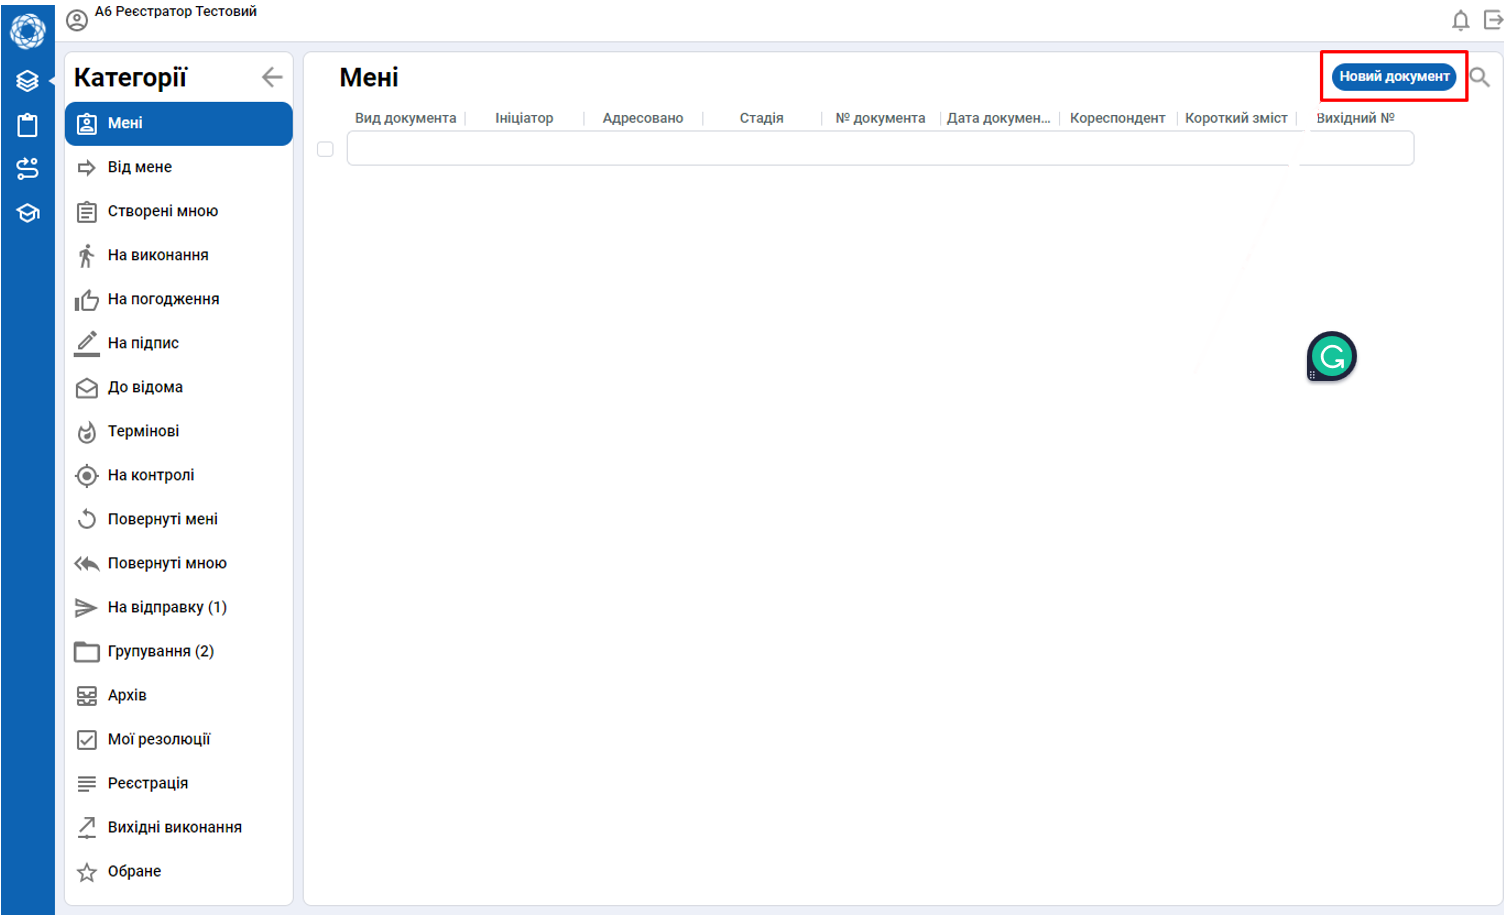
\includegraphics[width=\textwidth]{img/5.1.1.1.png}}
\caption{Рис. 5.1.1.1. Створення нового документа}
\end{figure}

--- Оберіть вид документа з переліку --- Вхідний документ (див. Рисунок 5.1.1.2)

\begin{figure}[!htbp]
\centerline{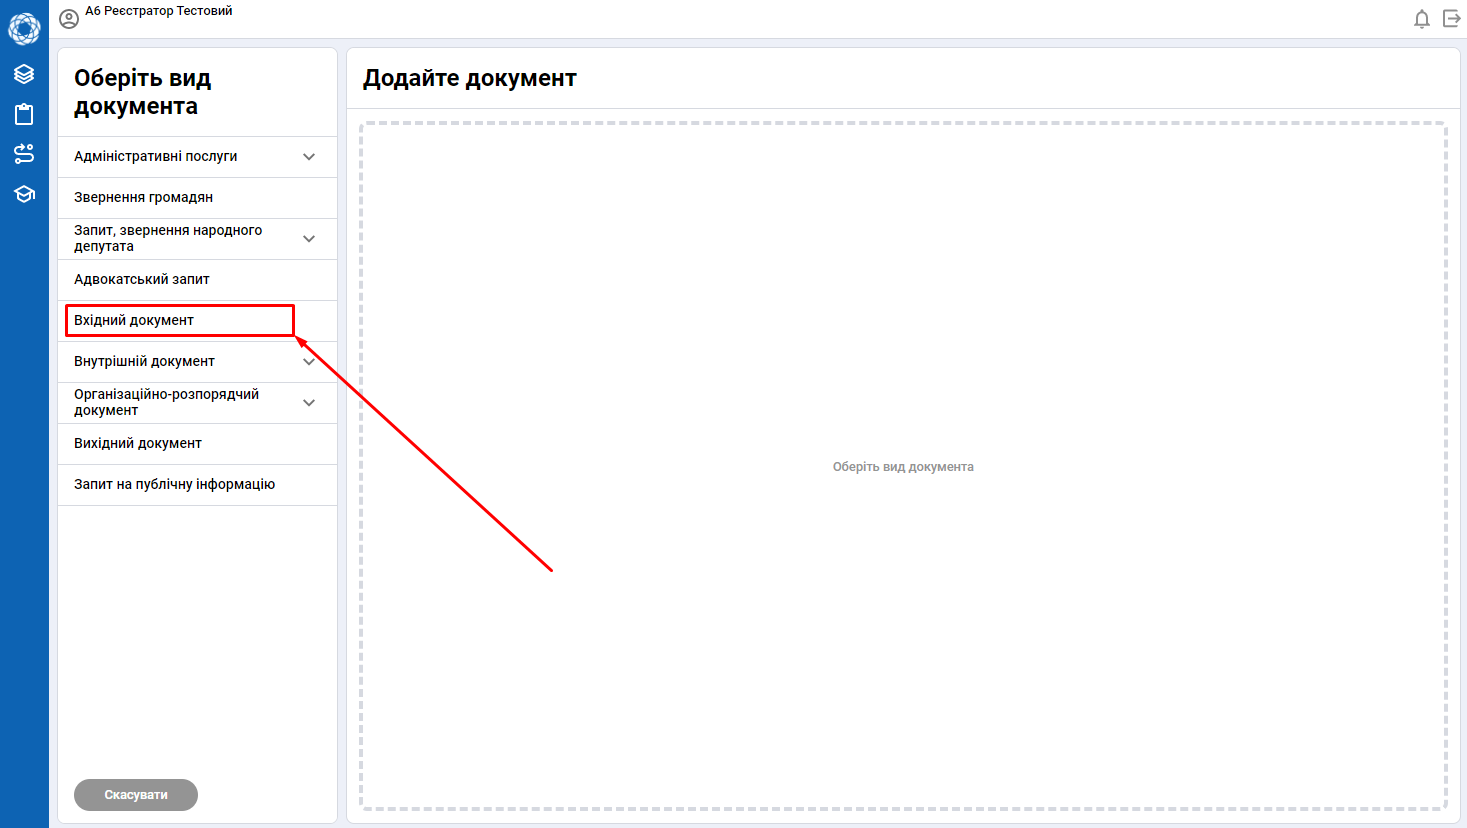
\includegraphics[width=\textwidth]{img/5.1.1.2.png}}
\caption{Рис. 5.1.1.2. Вибір виду документа}
\end{figure}

--- Заповніть РМК (область введення інформації позначена цифрою \circled{3} на
Рисунку 5.1.1.3 \circled{*} --- поле обов’язкове для заповнення)

\begin{figure}[!htbp]
\centerline{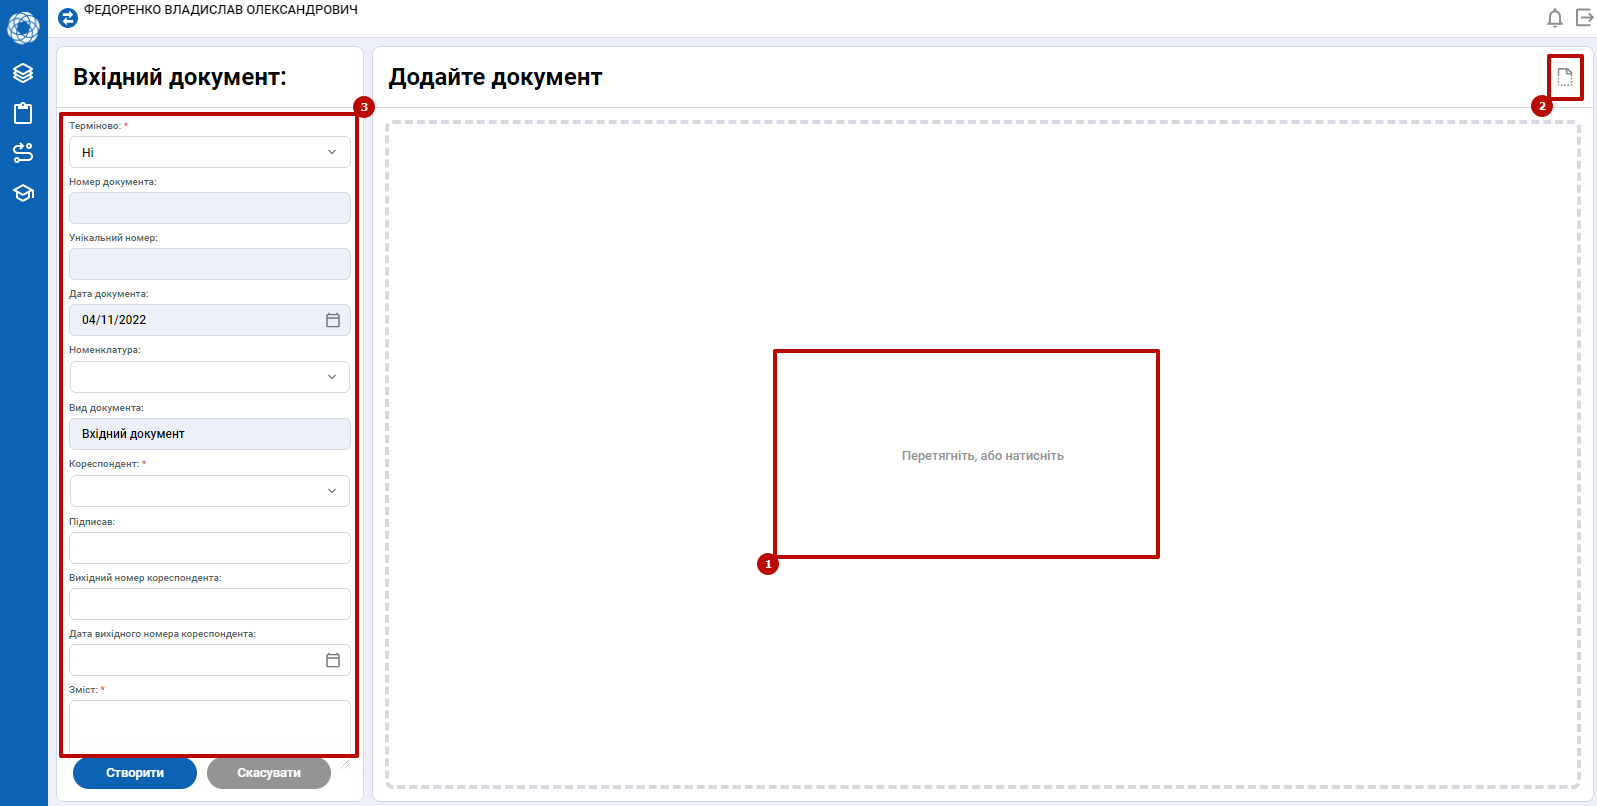
\includegraphics[width=\textwidth]{img/5.1.1.3.png}}
\caption{Рис. 5.1.1.3. Створення РМК}
\end{figure}

--- Додайте файл вхідного документа у зручний для Вас спосіб:
1) активний елемент «Перетягніть, або натисніть», позначений цифрою 1 на Рисунку 5.1.1.3;
2) шляхом сканування $\rightarrow$ піктограма 2 «Сканувати» у правому куті екранної форми (див. Рисунку 5.1.1.3).

\subsection{Сканування}

\subsection{Редагування}

\subsection{Визначення}

\section{Резолюція}

\subsection{Повернення документа на реєстрацію}

Для повернення вхідного документа на Реєстрацію:
--- натисніть активний елемент «Повернути» → позначено цифрою \circled{1} на Рисунку 5.2.1.1;
--- виберіть пункт «На реєстрацію» → позначено цифрою \circled{2}.

\begin{figure}[!htbp]
\centerline{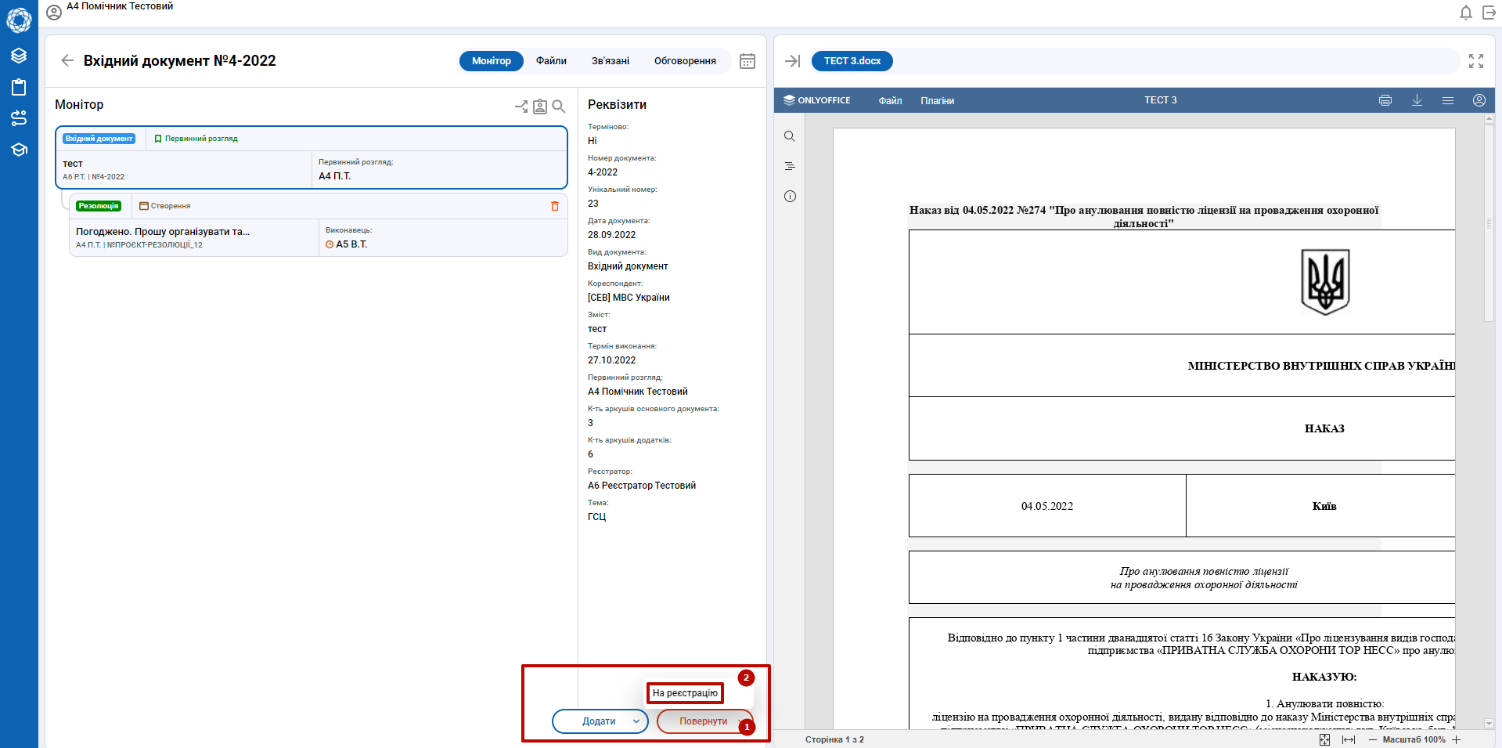
\includegraphics[width=\textwidth]{img/5.2.1.1.png}}
\caption{Рис. 5.2.1.1. }
\end{figure}

--- вкажіть причину повернення → \circled{1} «Змінити особу первинного розгляду» →
натисніть на кнопку, позначену цифрою \circled{2} на Рисунку 5.2.1.2.

\begin{figure}[!htbp]
\centerline{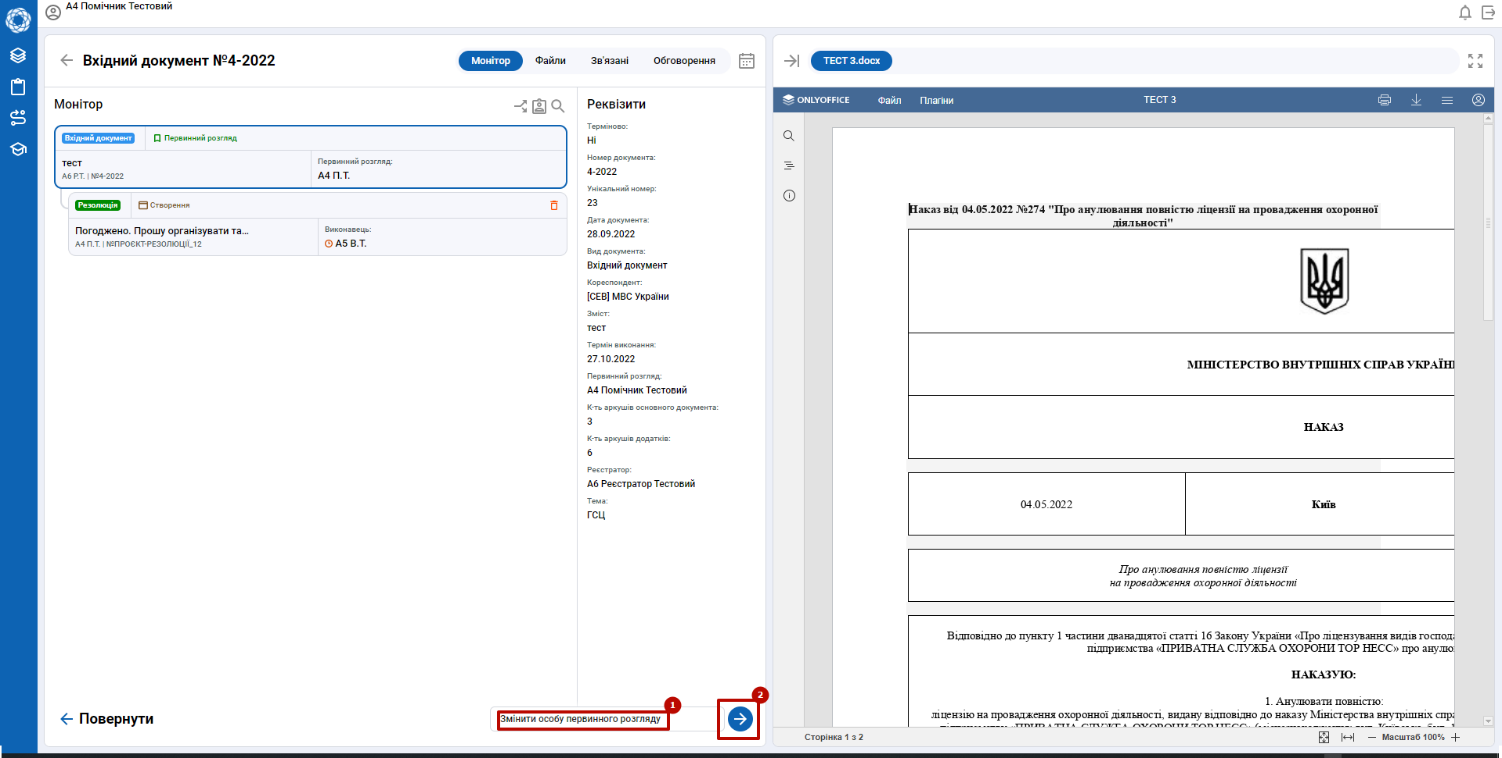
\includegraphics[width=\textwidth]{img/5.2.1.2.png}}
\caption{Рис. 5.2.1.2. Повернення документа на Реєстрацію}
\end{figure}

\subsection{Створення проєкту резолюції}

Для Створення проєкту резолюції помічник/ особа первинного розгляду/ посадова особа, яка отримала резолюцію (завдання):
--- натисніть активний елемент «Додати» → позначено цифрою 1 на Рисунку 5.2.2.1;
--- оберіть пункт «Резолюція» → позначено цифрою 2 на Рисунку 5.2.2.1.

\begin{figure}[!htbp]
\centerline{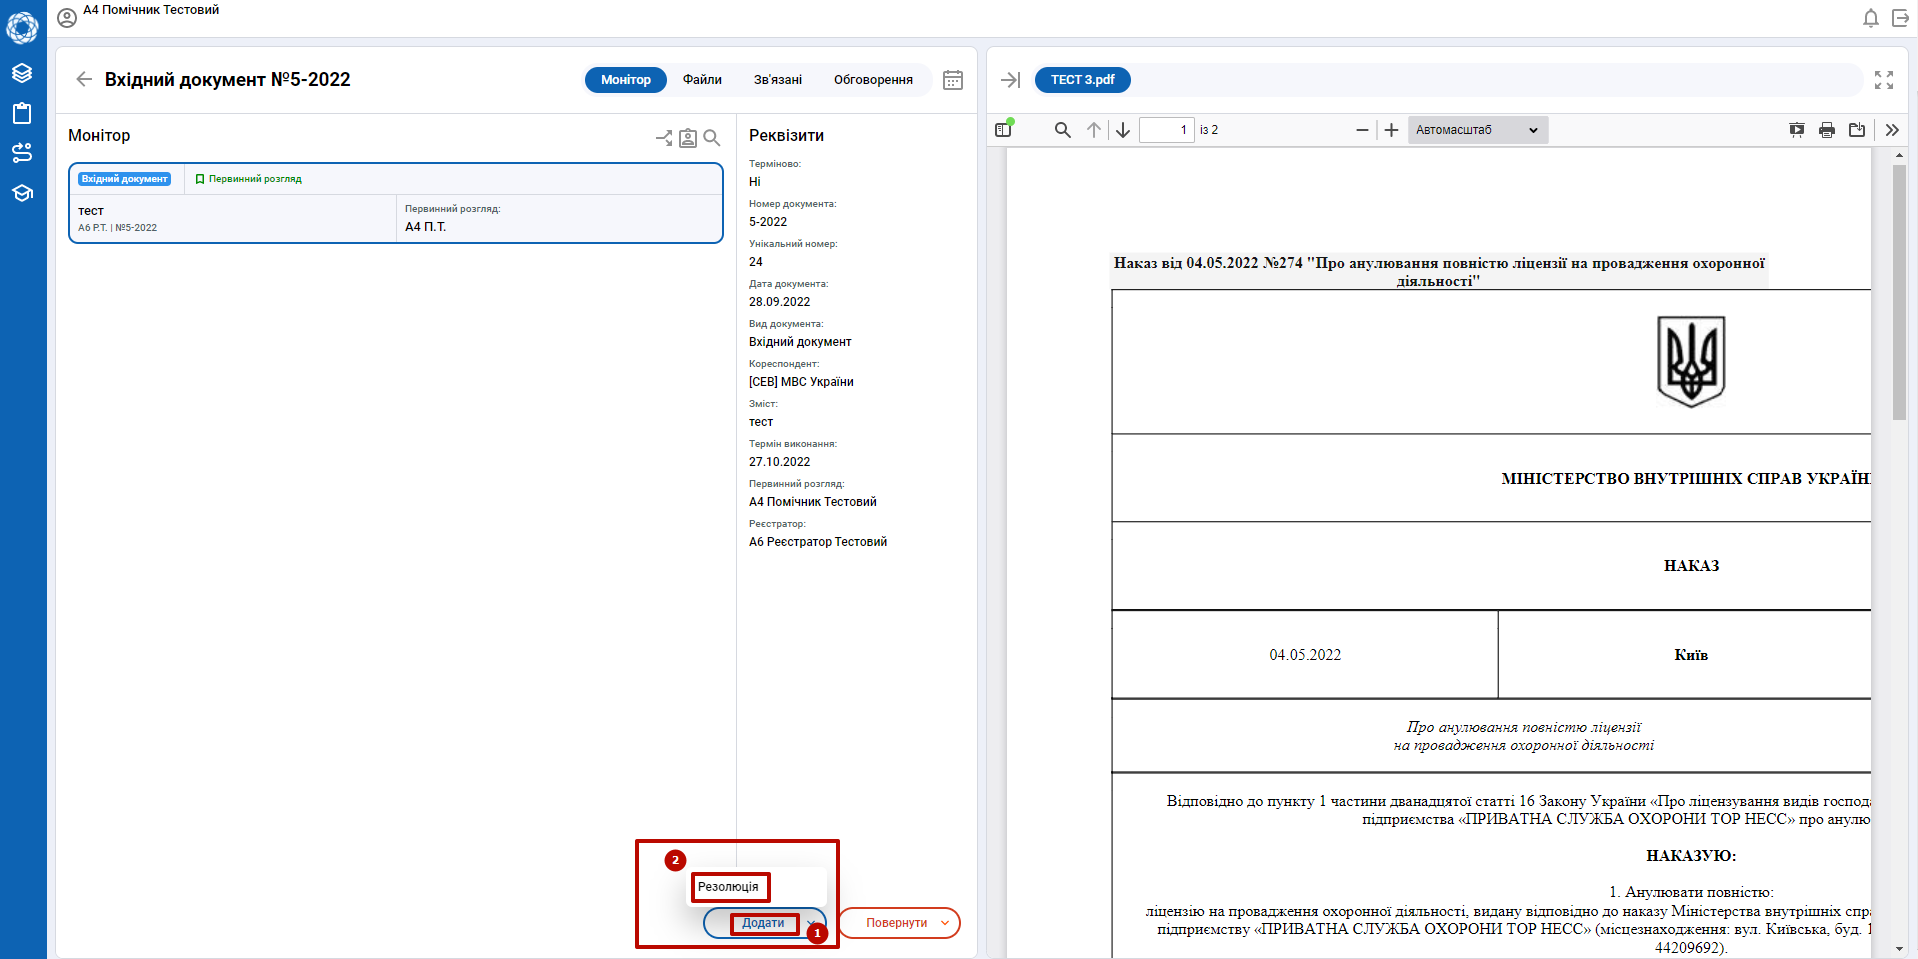
\includegraphics[width=\textwidth]{img/5.2.2.1.png}}
\caption{Рис. 5.2.2.1.}
\end{figure}

\subsection{Редагування/видалення проєкту резолюції}

\subsection{Підписання проєкту резолюції}

\subsection{Виконання/відхилення резолюції}

\section{Вихідний документ}

\subsection{Створення проєкту вихідного документу з резолюції}

\subsection{Редагування вихідного документу}

\subsection{Видалення проєкту вихідного документа}

\section{Внутрішній документ}

\subsection{Створення проєкту внутрішнього документа з резолюції}

\subsection{Редагування проєкту внутрішнього документу з резолюції}

\subsection{Видалення проєкту внутрішнього документу з резолюції}

\section{Організаційно-розпорядчі документи}

\subsection{Створення проєкта організаційно-розпорядчого документа}

\subsection{Редагування організаційно-розпорядчого документа}

\subsection{Видалення проєкта організаційно-розпорядчого документа}

\section{Пошук документів}

\section{Погодження проєкту документа}

\subsection{Редагування проєкту документа}

\subsection{Повернення проєкта документа}

\section{Групування}

\section{Проєкт відправки}

